\section{Problem 2A: SIR model}

\begin{figure}[htb]
	\centering
	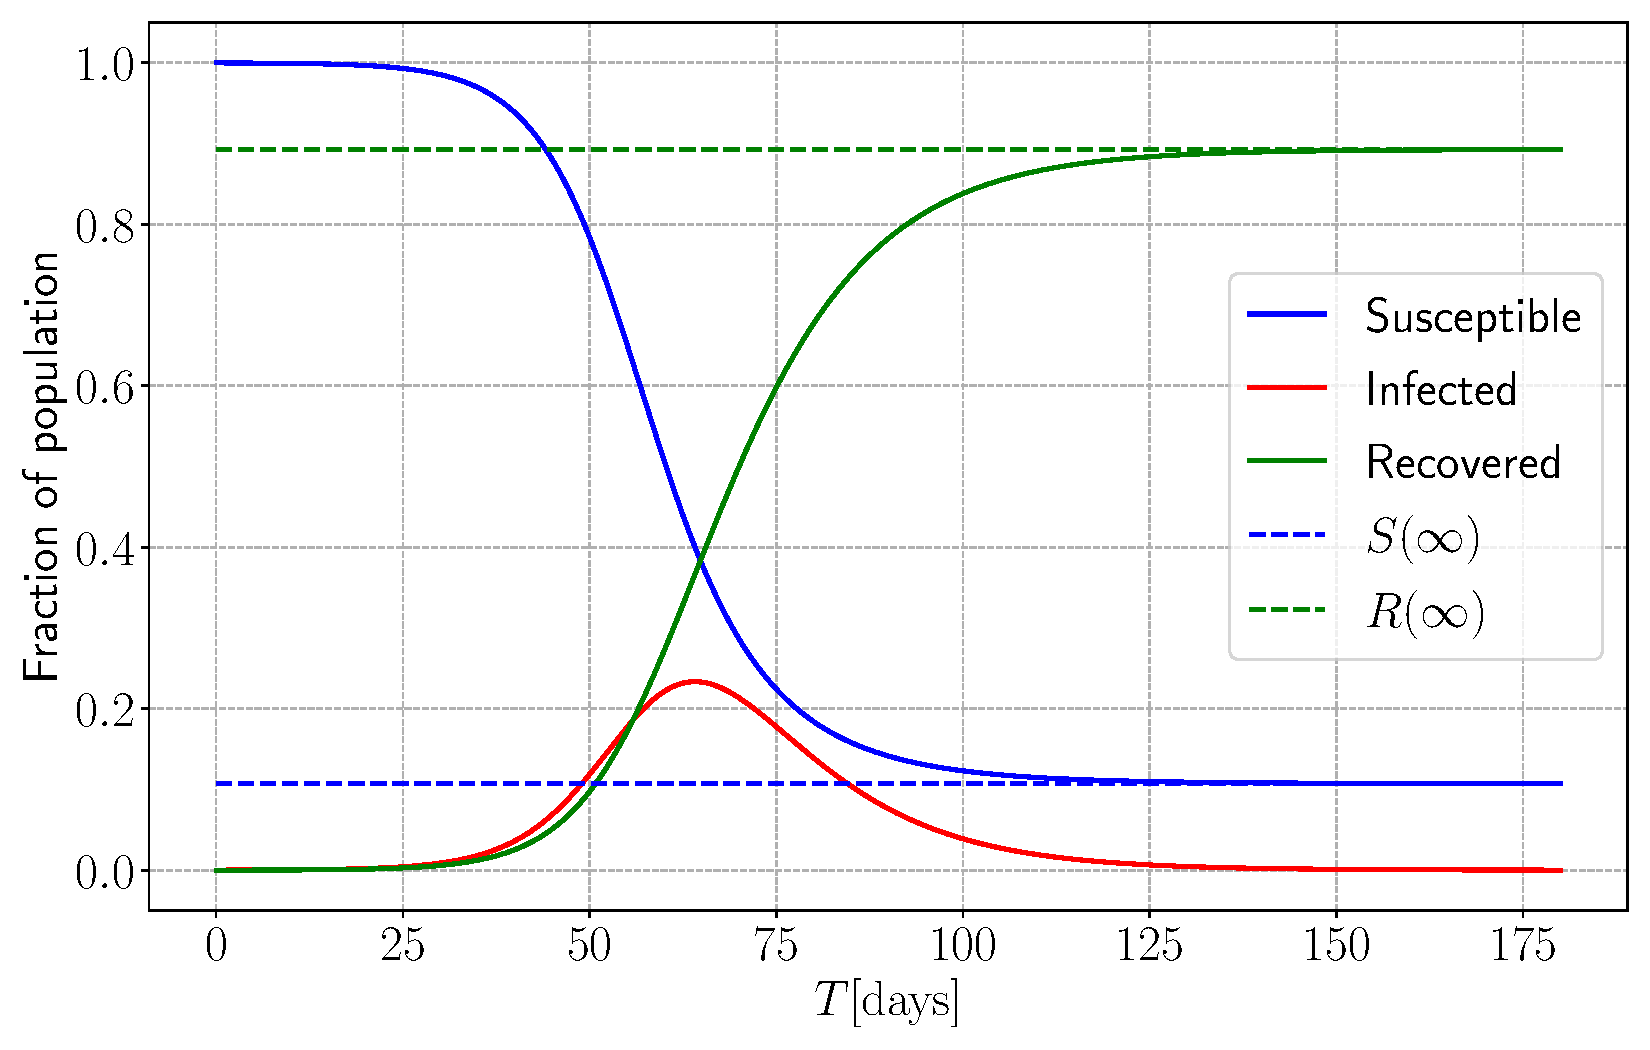
\includegraphics[width=0.8\columnwidth]{../fig/2Aa_SIR.pdf}
	\caption{SIR equations with $\beta = 0.25 \, \mathrm{day}^{-1}$, $\tau = 10 \, \mathrm{day}$.}
	\label{fig:SIR}
\end{figure}

\begin{figure}[htb]
	\centering
	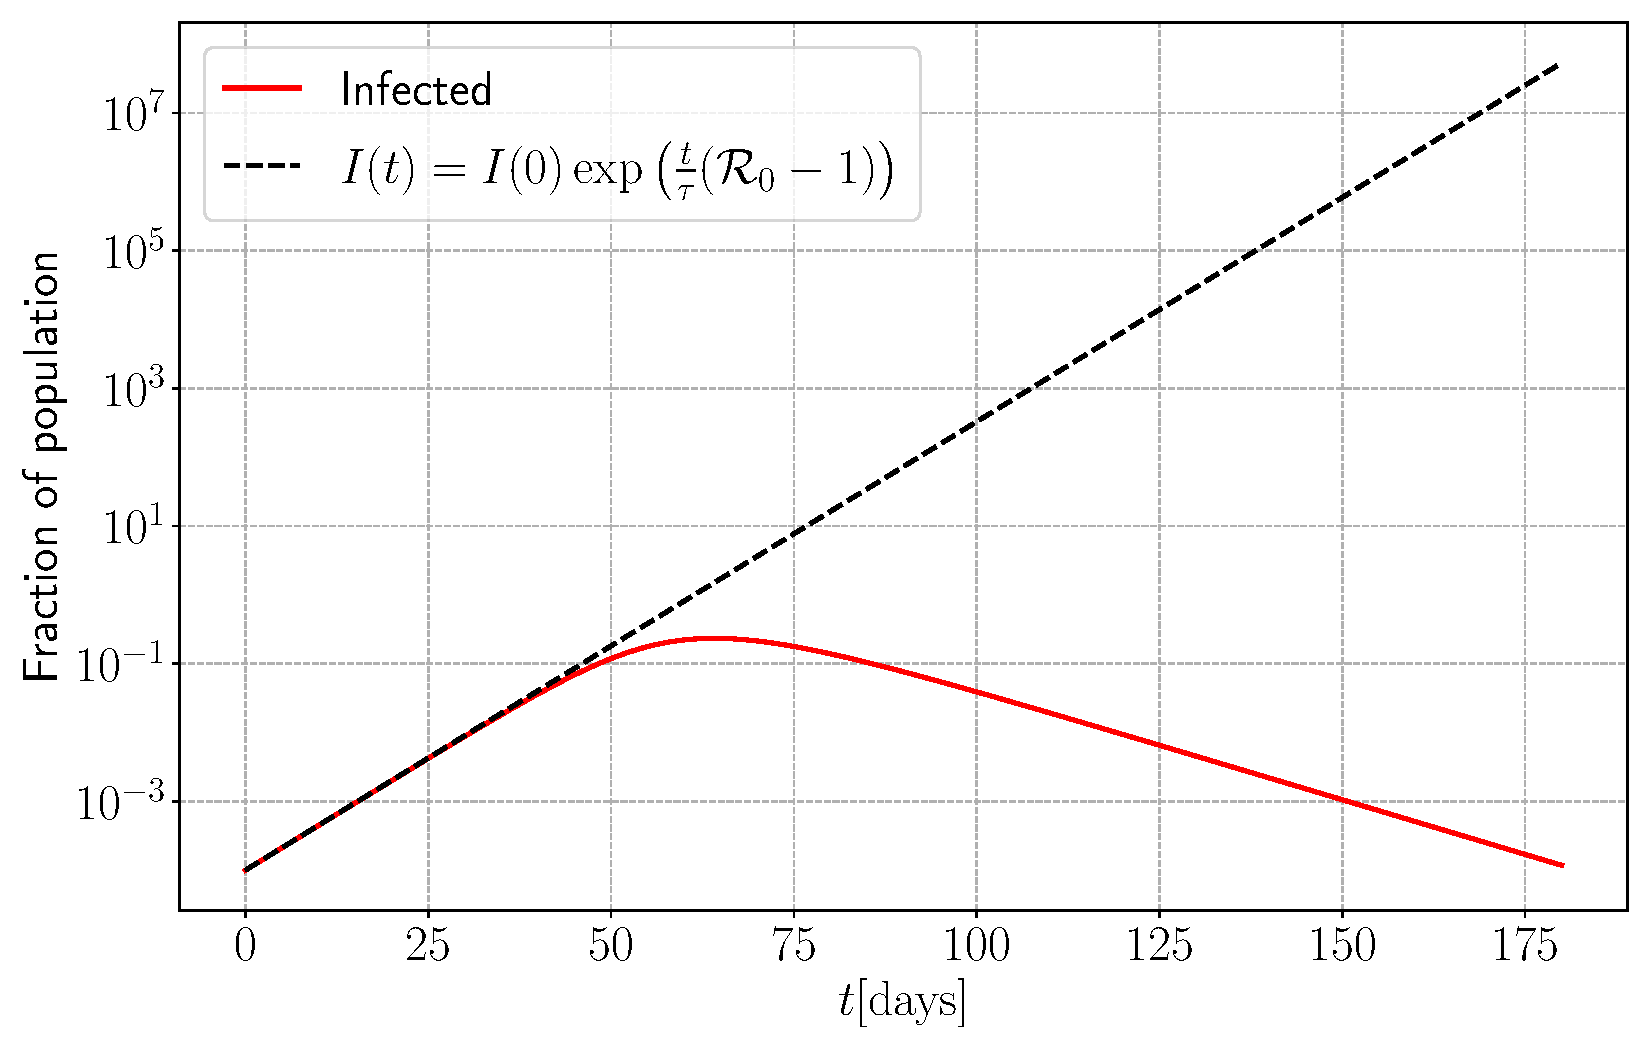
\includegraphics[width=0.8\columnwidth]{../fig/2Ab_I.pdf}
	\caption{Infected people compared with the analytical approximation at the early stages.}
	\label{fig:Infected}
\end{figure}

\begin{figure}[htb]
	\centering
	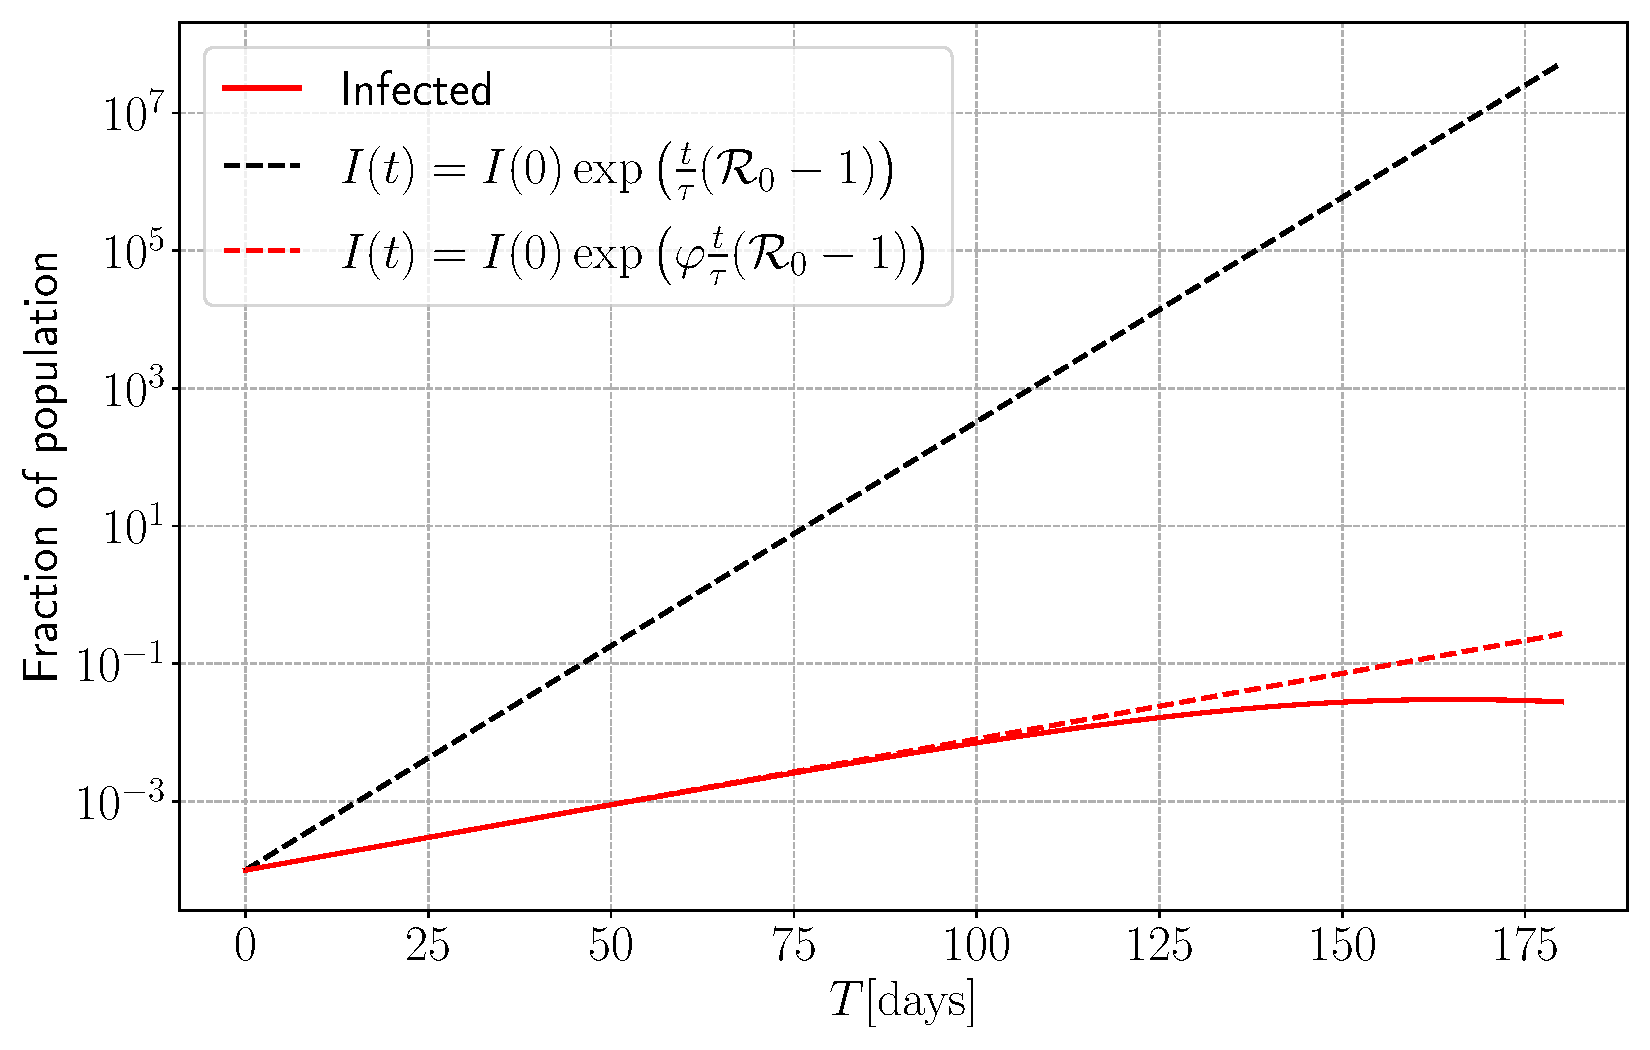
\includegraphics[width=0.8\columnwidth]{../fig/vac.pdf}
	\caption{The effect of vaccination, with $\varphi = 0.3$.}
	\label{fig:vaccination}
\end{figure}


\begin{table}[htb]
	\centering
	\caption{The maximum value of $\beta$ giving a peak less than $0.2$ of the infected fraction, and the minimum value of $R(0)$ (vaccinated) avoiding exponential growth.}
	\begin{tabular}{cccc}
		\toprule
		Parameter & value & $0.2 - \max_{t\in[0,\infty]} R(t)$ & Initial $\log$-slope \\
		\midrule
		$\beta$ & $0.28020370$ & $8.319\cdot 10^{-7}$ & --- \\
		$R(0)$  & $0.42410713$ & --- & $0.04393859$ \\
		\bottomrule
	\end{tabular}
\end{table}

